%
%  A presentation of ZMailer for  FUUG at SEA 2000 conference
%
%     FUUG = Finnish Unix User Group
%     SEA  = The baltic sea; cruising from Helsinki to Stockholm, and back
%
%  Matti Aarnio, 12-Sep-2000
%

\documentclass[a4paper,landscape]{slides}

\setlength{\topmargin}{-40pt}
\setlength{\headsep}{2EM}
\setlength{\footskip}{3\footskip}

\usepackage[dvips]{color}
\usepackage[dvips]{epsfig}
\usepackage{float}
\usepackage{wrapfig}
\usepackage{verbatim}

\newcommand{\SLIDEFOOT}{\centerline{\rm Matti Aarnio $<matti.aarnio@sonera.fi>$}}
\newcommand{\SLIDEHEAD}{\centerline{\tiny\rm FUUG @ SEA-2000:   ZMailer}}

\newcommand{\ZM}{ZMailer}

\begin{document}
\pagestyle{plain}

%%%%%%%%%%%%%%%%%%%%%%%%%%%%%%%%%%%%%%%%%%%%%%%%%%%%%%%%%%%%%%%%%

\begin{slide}

\begin{center}
 ZMailer --- A Different Kind of MTA
\end{center}

\vfill

\begin{center}
 
\epsfig{file=zmailer-logo.ps}
\end{center}

\vfill

\end{slide}

%%%%%%%%%%%%%%%%%%%%%%%%%%%%%%%%%%%%%%%%%%%%%%%%%%%%%%%%%%%%%%%%%

\begin{overlay}

\begin{center}
 ZMailer --- A Different Kind of MTA
\end{center}

\vfill

  A presentation of ZMailer for  FUUG at SEA 2000 conference

     FUUG = Finnish Unix User Group

     SEA  = The baltic sea; cruising from Helsinki to Stockholm, and back

 Matti Aarnio, 12-Sep-2000


\end{overlay}

%%%%%%%%%%%%%%%%%%%%%%%%%%%%%%%%%%%%%%%%%%%%%%%%%%%%%%%%%%%%%%%%%


\begin{slide}
\centerline{\large A bit of History}

\vfill
\ZM{} was created at {\it University of Toronto} around 1986 by
Mr. {\it Rayan Zachariassen} (hence the ``Z'' in the name.)

Rayan went to private sector around 1992, and $ZMailer$ development
was essentially abandoned by him.

Since then, yours truly has been hacking at it developing all kinds
of extensions for modern Internet email.

\vfill

\end{slide}

%%%%%%%%%%%%%%%%%%%%%%%%%%%%%%%%%%%%%%%%%%%%%%%%%%%%%%%%%%%%%%%%%


\begin{slide}

\centerline{\large \ZM{} structure}

\begin{wrapfigure}{l}{3in}
\mbox{
 \epsfig{file=zmprocs.ps,width=2.7in}
}
\end{wrapfigure}

\ZM{} consists of several main subsystems running in coordinated,
although separate existence.  This means also that any of the subsystems
can be shut down for a while without harming other subsystem functionality.

The task-transfer in between the subsystems is done via
the filesystem -- {``\it spool''}.

\vfill
\centerline{\it There are no suid-anything programs in this system!}

\vfill

\end{slide}

%%%%%%%%%%%%%%%%%%%%%%%%%%%%%%%%%%%%%%%%%%%%%%%%%%%%%%%%%%%%%%%%%


\begin{slide}

\centerline{\large \ZM{} structure}

\begin{wrapfigure}{l}{3in}
\mbox{
 \epsfig{file=zmprocs.ps,width=2.7in}
}
\end{wrapfigure}

Input subsystems: {\it sendmail, smtpserver, rmail, mail(3)} library

Routing subsystem: {\it router}

Delivery subsystem: {\it scheduler,} and {\it transport agents}

\vfill

\end{slide}

%%%%%%%%%%%%%%%%%%%%%%%%%%%%%%%%%%%%%%%%%%%%%%%%%%%%%%%%%%%%%%%%%


\begin{slide}

\centerline{\large \ZM{} subsystems: {\it ``POSTOFFICE/''}}

The \verb!$POSTOFFICE/! is \ZM{}'s way of referring to filesystem
where a few basic things are guaranteed to happen:
\begin{enumerate}
\item moving files around with {\it rename(2)} and/or {\it link(2), unlink(2)}
      works just fine in between different directories
\item i-node numbers are preserved over {\it rename(2)}, and {\it link(2)}
	system calls
\end{enumerate}

There are filesystems where these two things don't happen, e.g. possibly
{\it link(2)} can't be done in between directories.  Such ones are not
suitable for \ZM's \verb!$POSTOFFICE/! partition use.
\vfill

\end{slide}

%%%%%%%%%%%%%%%%%%%%%%%%%%%%%%%%%%%%%%%%%%%%%%%%%%%%%%%%%%%%%%%%%


\begin{slide}

\centerline{\large \ZM{} subsystems: {\it ``sendmail''}}

For normal local system use there needs to be a well-known
submission interface for email.  A de-facto one is {\it sendmail.}

\ZM's {\it sendmail} implements most of message submission options
of the real {\it sendmail(8).}

Many of {\it sendmail(8)} options are meaningless in \ZM{}, and thus
they are ignored, or in case of several administrative functions,
start subsystems in interactive test mode and/or just plain complain
loudly.

For message submission, \ZM's {\it sendmail} is extremely
{\it lightweight} one.  Just writing the message envelope and
message to the file, and moving it to {\it router} subsystem's care.



\vfill

\end{slide}

%%%%%%%%%%%%%%%%%%%%%%%%%%%%%%%%%%%%%%%%%%%%%%%%%%%%%%%%%%%%%%%%%


\begin{slide}

\centerline{\large \ZM{} subsystems: {\it ``smtpserver''}}

\begin{wrapfigure}{l}{5in}
\tiny
\begin{tabular}{ll}
ESMTP RFC's \\
1425/1651/2045 & EHLO framework \\
1426/1652 & 8BITMIME \\
1427/1653/1870 & SIZE \\
1830 & CHUNKING \\
1854/2197 & PIPELINING \\
1891 & DSN \\
1985 & ETRN \\
2034 & ENHANCEDSTATUSCODES \\
2487 & STARTTLS \\
2554+MS & AUTH LOGIN \\
2554+Netscape & AUTH=LOGIN
\end{tabular}
\end{wrapfigure}
\ZM's {\it smtpserver} subsystem implements a rich set of enhanced SMTP
features defined over the last 10 or so years.

At the same time it aims to be lightweight, fast protocol receiver with
ability to quickly verify incoming protocol stream syntax conformance,
but it can also be configured to behave sloppily in this regard.

\vfill

\end{slide}

%%%%%%%%%%%%%%%%%%%%%%%%%%%%%%%%%%%%%%%%%%%%%%%%%%%%%%%%%%%%%%%%%


\begin{overlay}
\small
\centerline{{\it ``smtpserver.conf''}}
\tiny

\begin{verbatim}
#
# smtpserver.conf - autogenerated edition
#
#PARAM maxsize              10000000    # Same as -M -option
#PARAM min-availspace           5000    # Minimum free in POSTOFFICE after
#                                       # message has arrived; in KILOBYTES.
#PARAM max-error-recipients        3    # More than this is propably SPAM!
#PARAM MaxSameIpSource            10    # Max simultaneous connections
#                                       # from any IP source address
#PARAM MaxParallelConnections    800    # Max simultaneous connections
#                                       # in total to the server
#PARAM TcpRcvBufferSize        32000    # Should not need to set!
#PARAM TcpXmitBufferSize       32000    # Should not need to set!
#
#PARAM ListenQueueSize            10    # listen(2) parameter
#
#PARAM RcptLimitCount          10000    # Max number of recipients for one
#                                       # MAIL FROM session. Minimum: 100
#
#PARAM use-tcp-wrapper                  # Use tcp-wrapper in addition to
#                                       # actual input policy controls.
\end{verbatim}
\end{overlay}
\begin{overlay}
\small
\centerline{{\it ``smtpserver.conf''}}
\tiny
\begin{verbatim}
#PARAM BindPort                   25    # Binding port
#PARAM BindAddress         [0.0.0.0]    # Binding address - for multihomers..
#PARAM BindAddress       [IPv6.0::0]    # and here is for IPv6 - NO SPACES!
#
# Enables of some commands:
PARAM   DEBUGcmd
PARAM   EXPNcmd
PARAM   VRFYcmd
PARAM   enable-router   # This is a security decission for you.
#                       # This is needed for EXPN/VRFY and interactive
#                       # processing of MAIL FROM and RCPT TO addresses.
#                       # However it also may allow external user entrance
#                       # to ZMailer router shell environment with suitably
#                       # pervert input, if quotation rules are broken in
#                       # the scripts.
\end{verbatim}
\end{overlay}
\begin{overlay}
\small
\centerline{{\it ``smtpserver.conf''}}
\tiny
\begin{verbatim}
PARAM   smtp-auth       # enable if you want to allow SMTP to autenticate
#                       # with the default code against system  /etc/passwd
#                       # (or whatever source  getpwnam() uses for it..)
#
PARAM  AUTH-LOGIN-also-without-TLS
#                       # Enable, if the "AUTH LOGIN" is to be allowed to
#                       # be used without running under SSL/TLS security
#                       # envelope.
#
#PARAM  MSA-mode        # Message Submission Agent mode. Require
#                       # successful user authentication during SMTP
#                       # sessions initiated from outside of the trusted
#                       # networks or the networks with relaying enabled
#                       # (see "fulltrustnet" and "relaycustnet" in
#                       # smtp-policy.src file).
#
PARAM   deliverby 60
#                       # RFC 2852 defined deliverby machinery.
\end{verbatim}
\end{overlay}
\begin{overlay}
\small
\centerline{{\it ``smtpserver.conf''}}
\tiny
\begin{verbatim}
#PARAM  SMTP-auth-pipe /path/to/program
#                       # External authentication program. The
#                       # authenticator should read a username from
#                       # command line and a password from standard input.
#                       # Exit status 0 means successful authentication.
#
# Disablers of some facility adverticements
#PARAM  NoEHLO
#PARAM  NoPIPELINING
#PARAM  No8BITMIME
PARAM   NoCHUNKING
#PARAM  NoDSN
#PARAM  NoETRN
PARAM  no-multiline-replies # except to EHLO (Bloody M$ RFC821/AppE violators)
\end{verbatim}
\end{overlay}
\begin{overlay}
\small
\centerline{{\it ``smtpserver.conf''}}
\tiny
\begin{verbatim}
# HDR220 metatags:
#  %% -- '%' character
#  %H -- SS->myhostname
#  %I -- '+IDENT' if 'identflg' is set
#  %V -- VersionNumb
#  %T -- curtime string
#  %X -- xlatelang parameter
#
#PARAM hdr220 %H ZMailer ESMTP-server %V running at Yoyodyne Propulsion Inc
#PARAM hdr220 %H ESMTP (NO UCE)(NO UBE) our local time is now %T
#
# Note above the "ESMTP" words are present because *some* MTA systems won't
# do EHLO greeting, unless they see "ESMTP" - against RFC 1869 part 4.
# "EHLO is to be done blindly, server responses are not to be studied for
#  any possible 'ESMTP' keyword!"
\end{verbatim}
\end{overlay}
\begin{overlay}
\small
\centerline{{\it ``smtpserver.conf''}}
\tiny
\begin{verbatim}
PARAM help -------------------------------------------------------------
PARAM help  This mail-server is at Yoyodyne Propulsion Inc.
PARAM help  Our telephone number is: +1-234-567-8900, and
PARAM help  telefax number is: +1-234-567-8999
PARAM help  Our business-hours are Mon-Fri: 0800-1700 (Timezone: -0700)
PARAM help
PARAM help  Questions regarding our email service should be sent via
PARAM help  email to address  <postmaster@OURDOMAIN>
PARAM help  Reports about abuse are to be sent to: <abuse@OURDOMAIN>
PARAM help -------------------------------------------------------------
#
# Uncomment following for not to strip incoming addresses of format:
# <@aa,@bb:cc@dd> into non-source-routed base form: <cc@dd>
#
#PARAM  allowsourceroute # DON'T ENABLE UNLESS YOU USE ROUTER BASED
#                        # POLICY ANALYSIS!
#
# The policy database:  (NOTE: See  'makedb'  for its default suffixes!)
#
PARAM  policydb   btree  /opt/mail/db/smtp-policy
\end{verbatim}
\end{overlay}
\begin{overlay}
\small
\centerline{{\it ``smtpserver.conf''}}
\tiny
\begin{verbatim}
#PARAM  tarpit 0 0   # No "tarpit" for 4XX/5XX reply codes
#PARAM  tarpit 20 2  # Initial delay: 20 secs, next = prev + (prev * 2)

#
# TLSv1/SSLv[23] parameters; all must be used for the system to work!
#
# See  http://www.aet.tu-cottbus.de/personen/jaenicke/pfixtls/doc/setup.html
#
PARAM   use-tls
PARAM   tls-CAfile      /opt/mail/db/smtpserver-CAcert.pem
PARAM   tls-cert-file   /opt/mail/db/smtpserver-cert.pem
PARAM   tls-key-file    /opt/mail/db/smtpserver-key.pem
#  # If system default SSL-session-cache is to be used ?
PARAM   tls-use-scache
PARAM   tls-scache-timeout 3600 # (cache timeout in seconds)
#  # Then some futher thoughs that may materialize some time..
#PARAM tls-loglevel     0
#PARAM tls-ccert-vd     0
#PARAM tls-ask-cert     0
#PARAM tls-require-cert 0
##PARAM tls-CApath ... (somewhen: ways to verify client's certificates)
##PARAM tls-enforce-tls 1
\end{verbatim}
\end{overlay}
\begin{overlay}
\small
\centerline{{\it ``smtpserver.conf''}}
\tiny
\begin{verbatim}
#
# Elements to be added into "Received:" header's initial comment part:
#
PARAM rcvd-ident        # The ident lookup result (or even admitting it)
PARAM rcvd-whoson       # Likewise for "whoson"
PARAM rcvd-auth-user    # Authenticated Username
PARAM rcvd-tls-mode     # Cipher, or not
PARAM rcvd-tls-ccert    # Client Certificate reference

PARAM etrn-cluster  localhost        etrn zzETRNzz
PARAM etrn-cluster  ipv6-localhost   etrn zzETRNzz
\end{verbatim}
\end{overlay}
\begin{overlay}
\small
\centerline{{\it ``smtpserver.conf''}}
\tiny
\begin{verbatim}
#
#
# HELO/EHLO-pattern     style-flags (Remember: 'ftve' set needs enable-router!)
#               [max loadavg]
#
localhost           999 ftveR
some.host.domain    999 !NO EMAIL ACCEPTED FROM YOUR MACHINE
# If the host presents itself as:  HELO [1.2.3.4], be lenient to it..
# The syntax below is due to these patterns being SH-GLOB style patterns
# where the brackets are special characters.
\[*\]               999 ve
# Per default demant strict syntactic adherence, including fully
# qualified addresses for  MAIL FROM, and RCPT TO.  To be lenient
# on that detail, remove the "R" from "veR" string below:
*                   999 veR

\end{verbatim}
%\vfill

\end{overlay}

%%%%%%%%%%%%%%%%%%%%%%%%%%%%%%%%%%%%%%%%%%%%%%%%%%%%%%%%%%%%%%%%%


\begin{slide}

\centerline{\large \ZM{} subsystems: {\it ``router''}}

- about the router program tasks

- about router configuration mechanisms

- about the router script language


\vfill

\end{slide}

%%%%%%%%%%%%%%%%%%%%%%%%%%%%%%%%%%%%%%%%%%%%%%%%%%%%%%%%%%%%%%%%%


\begin{slide}

\centerline{\large \ZM{} subsystems: {\it ``scheduler''}}

\vfill

\end{slide}

%%%%%%%%%%%%%%%%%%%%%%%%%%%%%%%%%%%%%%%%%%%%%%%%%%%%%%%%%%%%%%%%%

\begin{overlay}

\centerline{\large \ZM{} subsystems: {\it ``scheduler.conf''}}

\vfill

\end{overlay}

%%%%%%%%%%%%%%%%%%%%%%%%%%%%%%%%%%%%%%%%%%%%%%%%%%%%%%%%%%%%%%%%%

\begin{overlay}

\centerline{\large \ZM{} subsystems: {\it ``scheduler.auth''}}

\vfill

\end{overlay}

%%%%%%%%%%%%%%%%%%%%%%%%%%%%%%%%%%%%%%%%%%%%%%%%%%%%%%%%%%%%%%%%%

\begin{slide}

\centerline{\large \ZM{} subsystems: {\it ``mailq''}}

\vfill

\end{slide}

%%%%%%%%%%%%%%%%%%%%%%%%%%%%%%%%%%%%%%%%%%%%%%%%%%%%%%%%%%%%%%%%%


\begin{slide}

\centerline{\large \ZM{} subsystems: {\it ``mailbox''}}

\vfill

\end{slide}

%%%%%%%%%%%%%%%%%%%%%%%%%%%%%%%%%%%%%%%%%%%%%%%%%%%%%%%%%%%%%%%%%


\begin{slide}

\centerline{\large \ZM{} subsystems: {\it ``smtp''}}

\vfill

\end{slide}

%%%%%%%%%%%%%%%%%%%%%%%%%%%%%%%%%%%%%%%%%%%%%%%%%%%%%%%%%%%%%%%%%


\begin{slide}

\centerline{\large \ZM{} subsystems: {\it ``sm, error, hold''}}

\vfill

\end{slide}

%%%%%%%%%%%%%%%%%%%%%%%%%%%%%%%%%%%%%%%%%%%%%%%%%%%%%%%%%%%%%%%%%


\end{document}
